\documentclass{article}
\usepackage{graphicx}
\usepackage{geometry}
\usepackage[colorlinks = true,
            linkcolor = blue,
            urlcolor  = blue,
            citecolor = blue,
            anchorcolor = blue]{hyperref}
 \geometry{
 a4paper,
 left=20mm,
 top=20mm,
 bottom=20mm
 }
\begin{document}
	In this document, we mainly discuss the result from Python simulation for two Magnetic Traps widely used by Magneto Optical Traps. Simulation results are present below, while the python code can be found in my personal repository at \href{https://github.com/YJ-Yuan}{THIS LINK}. We analyze the trap used in NPQO and described by "A dark-line two-dimensional magneto-optical trap of 85Rb atoms with high optical depth". X direction in our simulation is the axis of symmetry, while Z and Y are cross sectional axes. 
	
	In NPQO, 1.5A current is used for the magnetic loop while in the paper, 70A instead. In NPQO, multiple wounds are present while in the paper, only one wound(they can also make them to be multiple, but not like the one in NPQO which has more than 100 wounds), which also has an advantage: because the core is magnetic material, it can be shut down for a while while keeping the magnetic field. It can also be replaced by a magnet. 
	
\begin{figure*}[h]
	\centering
	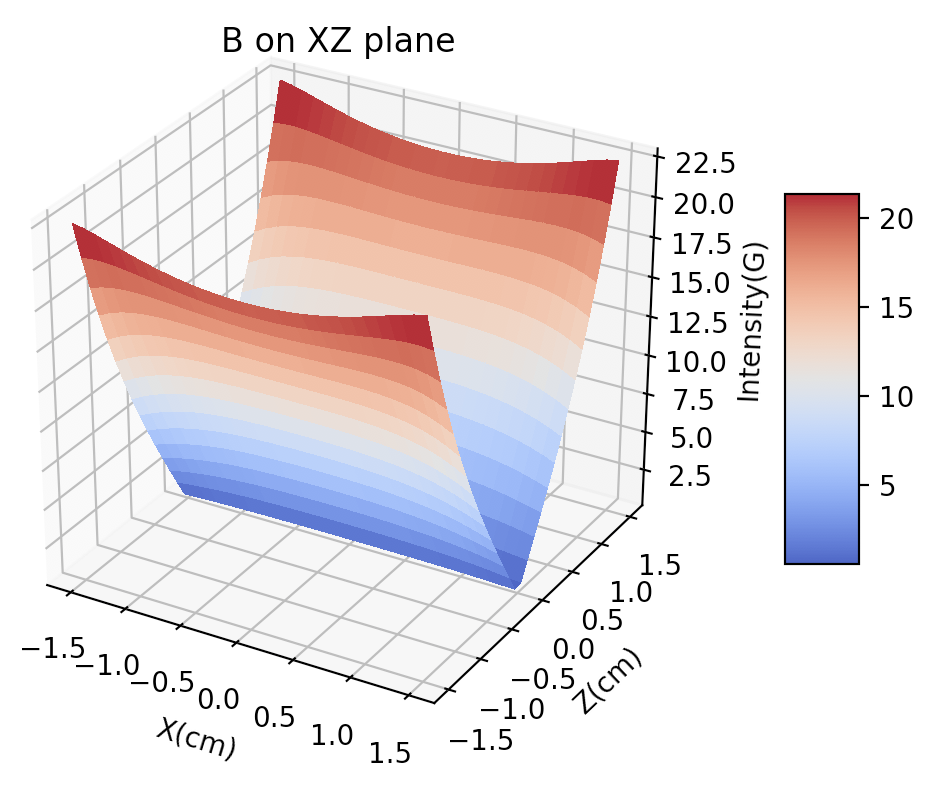
\includegraphics[scale=0.5]{MOTXZ}
	\caption{Their intensity of magnetic field aross section(XZ plane)}
\end{figure*}
\begin{figure*}[h]
	\centering
	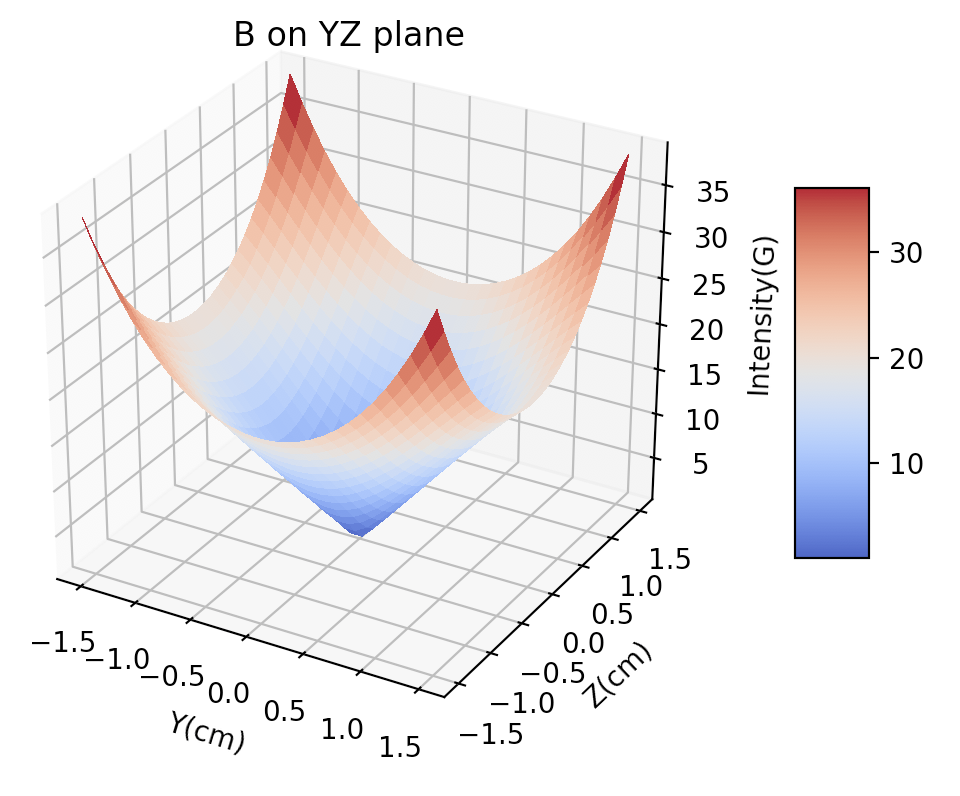
\includegraphics[scale=0.5]{MOTYZ}
	\caption{Their intensity of magnetic field aross section(YZ plane)}
\end{figure*}
\begin{figure*}[h]
	\centering
	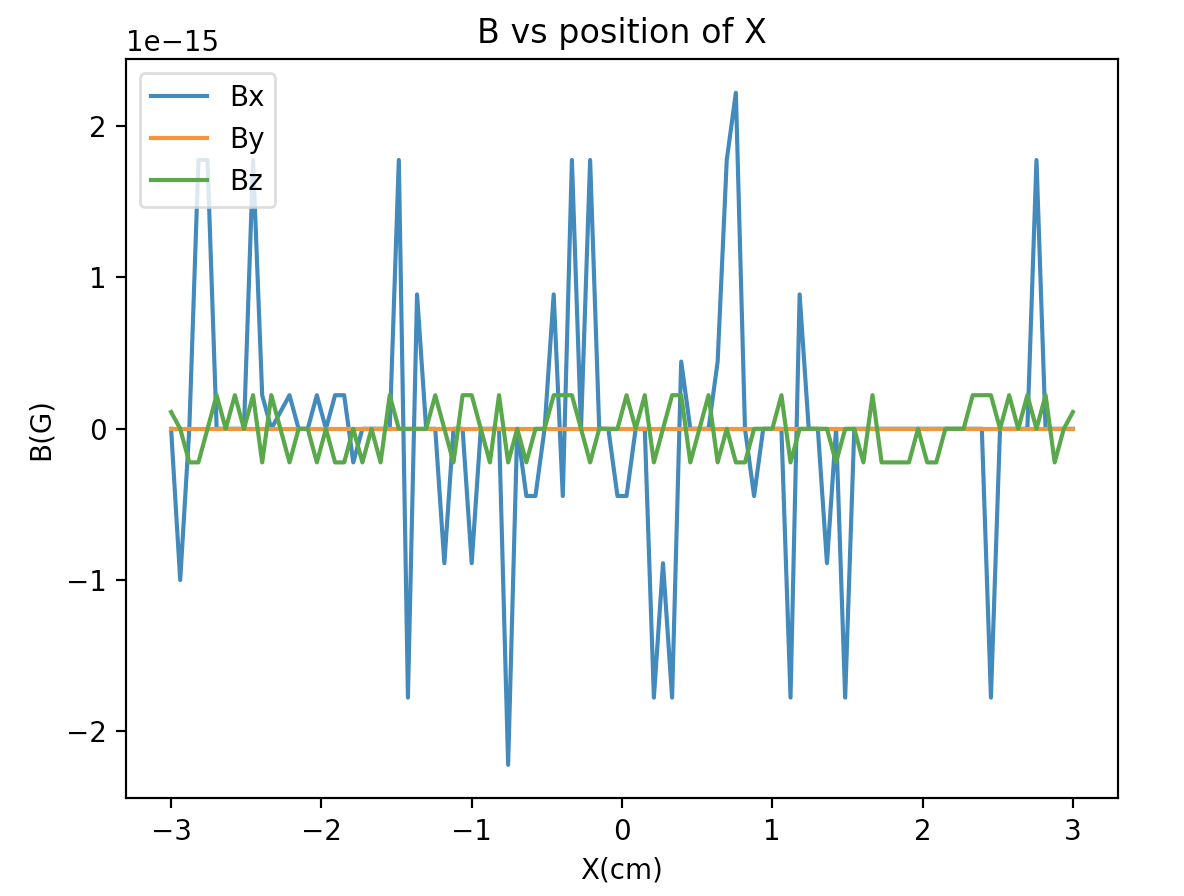
\includegraphics[scale=0.45]{MOTBx}
	\caption{Their components of B to x, y and z directions along x-axis}
\end{figure*}

\begin{figure*}[h]
	\centering
	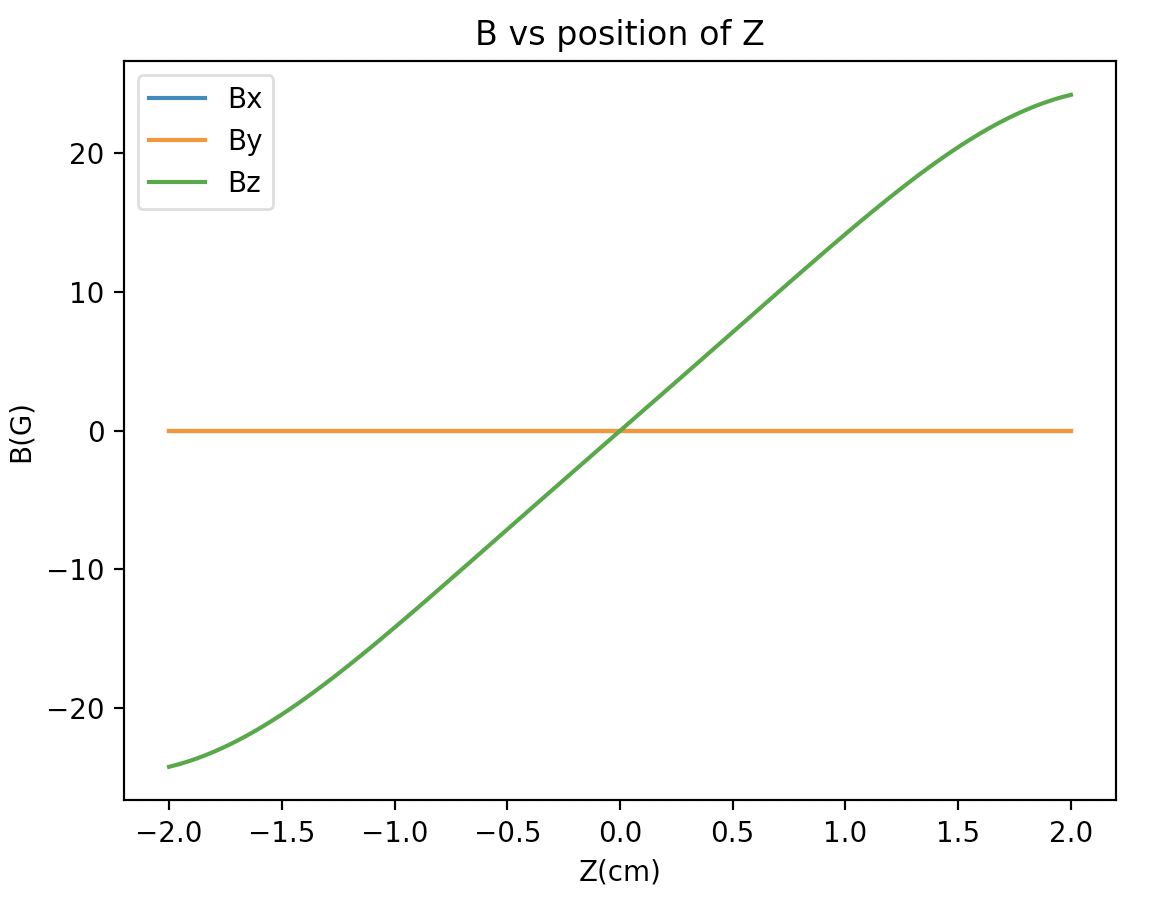
\includegraphics[scale=0.45]{MOTBz}
	\caption{Their components of B to x, y and z directions along z-axis}
\end{figure*}

\begin{figure*}[h]
	\centering
	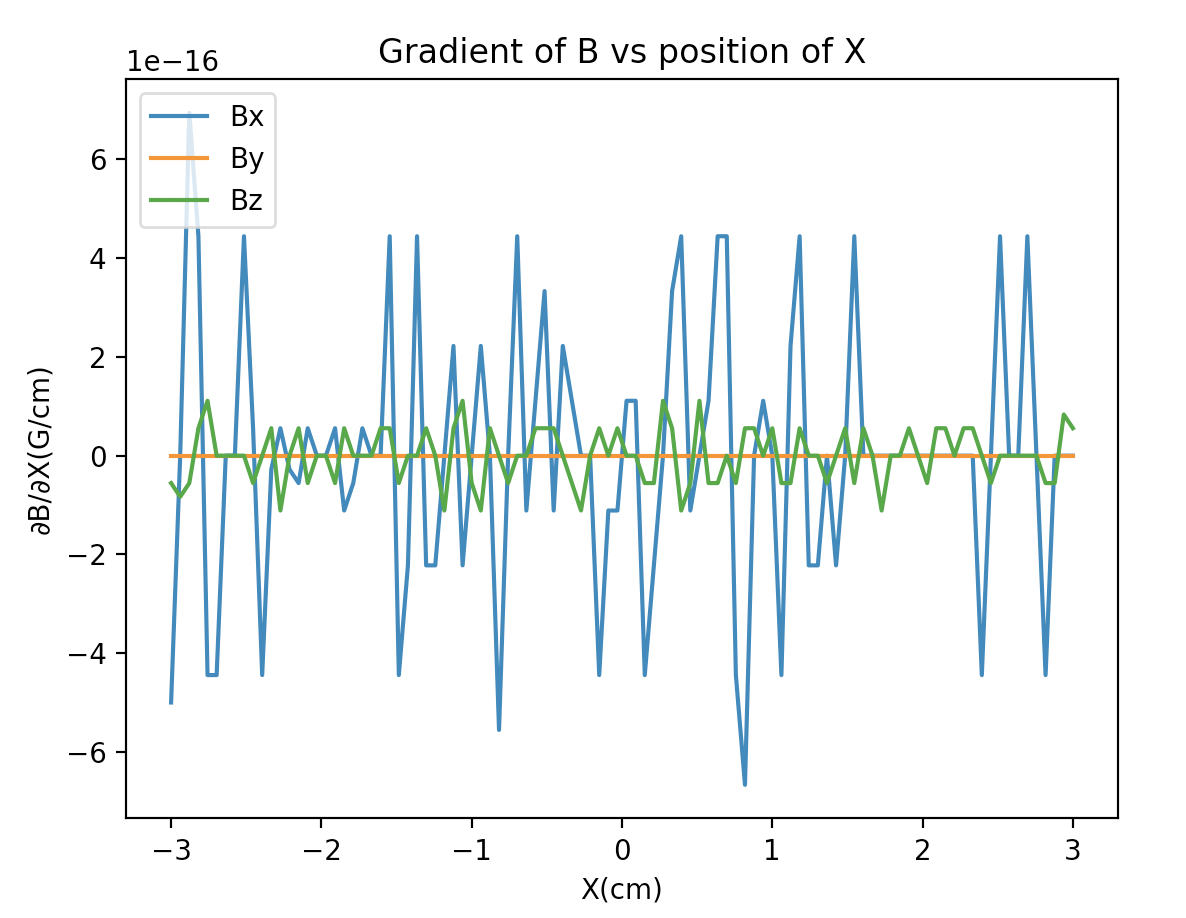
\includegraphics[scale=0.45]{MOTGradx}
	\caption{Their components of gradient of B to x, y and z directions along x-axis}
\end{figure*}

\begin{figure*}[h]
	\centering
	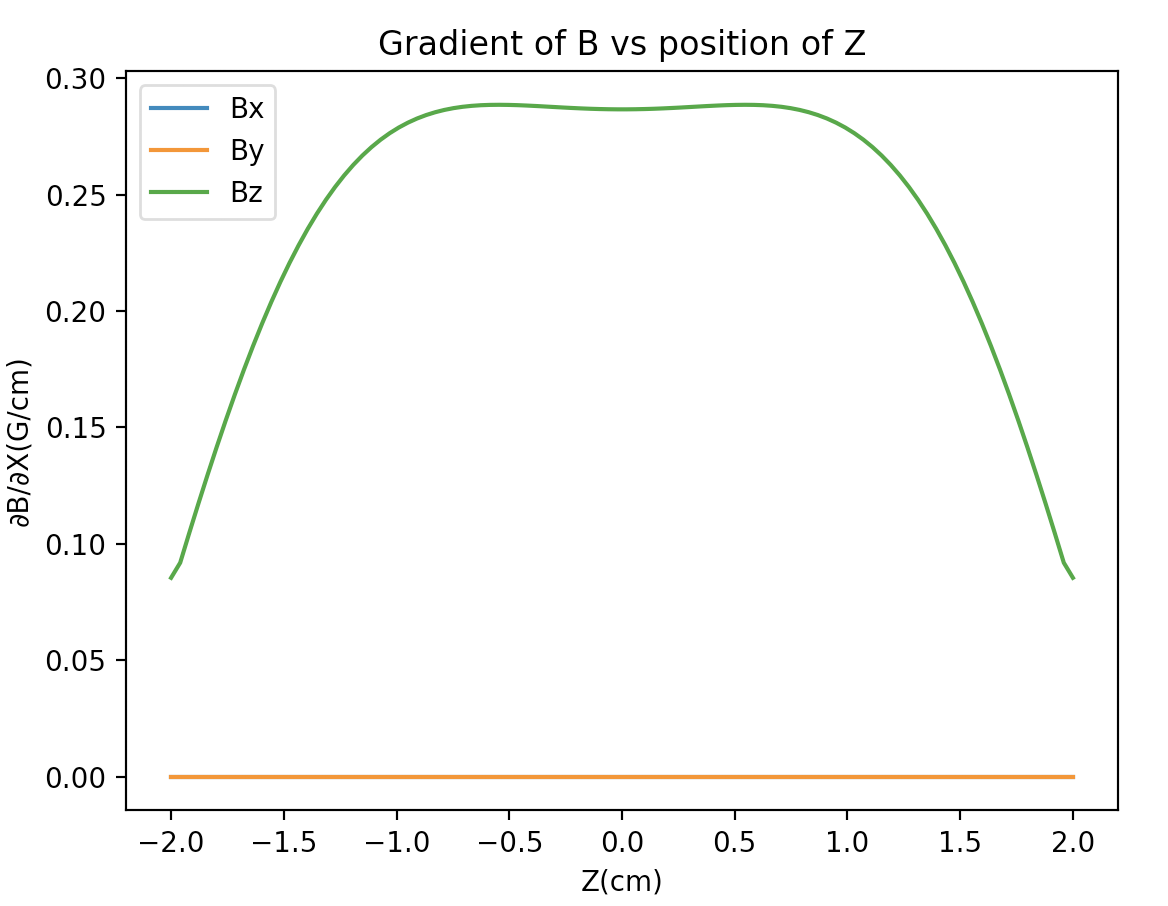
\includegraphics[scale=0.45]{MOTGradz}
	\caption{Their components of gradient of B to x, y and z directions along z-axis}
\end{figure*}

\begin{figure*}[h]
	\centering
	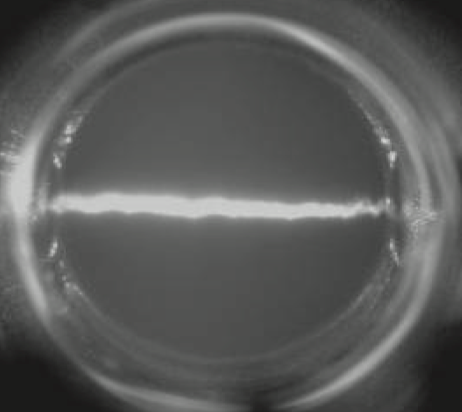
\includegraphics[scale=0.5]{theirRes}
	\caption{Compared to their result, in which the length of Z direction(in their paper they call this axis X or Y) is 1.7cm(make sense) Although I cannot re-establish their result which has gradient ~1G/cm. In my simulation it is 0.2G/cm. So I assume they use multiple wounds instead of one. And their setup is more likely a Linear Trap..?}
\end{figure*}

\begin{figure*}[h]
	\centering
	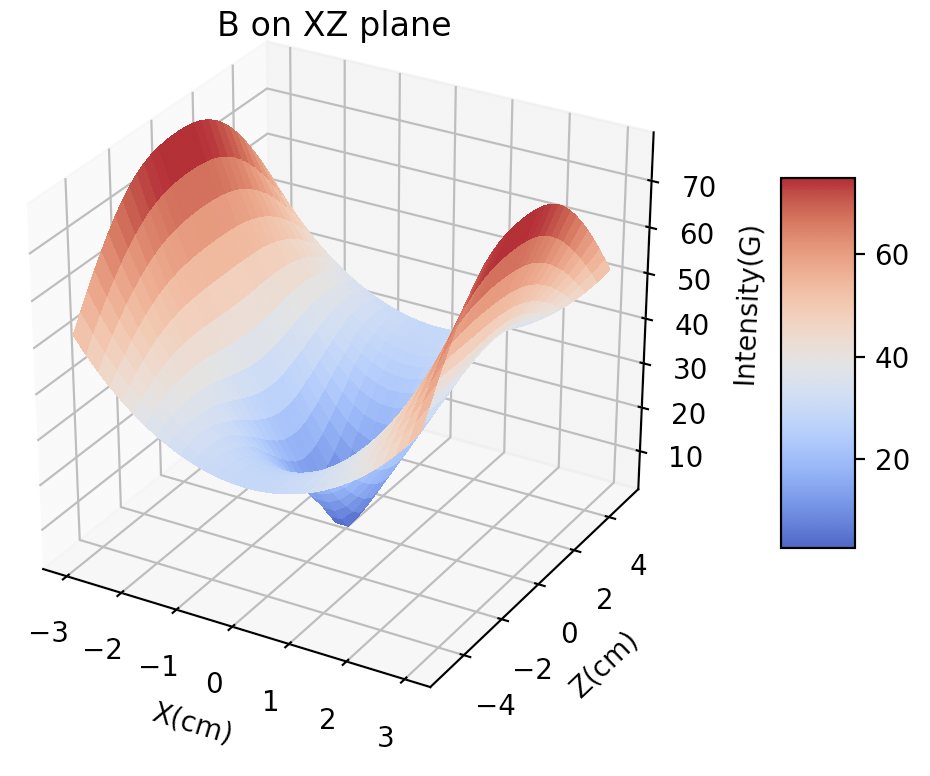
\includegraphics[scale=0.5]{OurXZ}
	\caption{In our lab, Intensity of magnetic field aross section(XZ plane)}
\end{figure*}
\begin{figure*}[h]
	\centering
	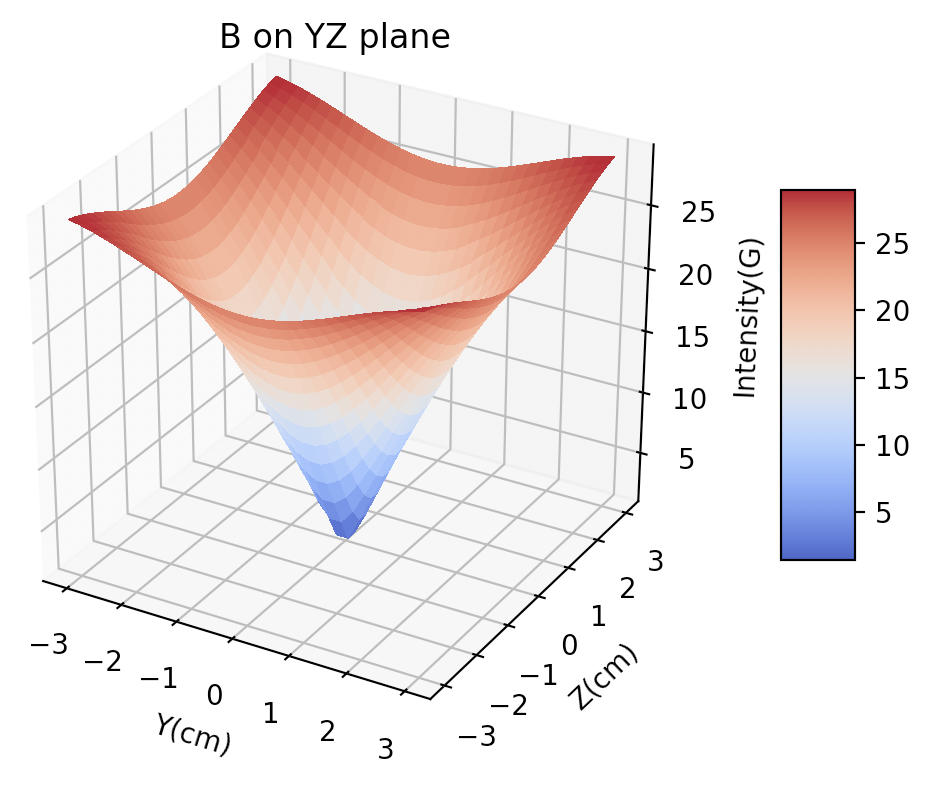
\includegraphics[scale=0.5]{OurYZ}
	\caption{In our lab, Intensity of magnetic field aross section(YZ plane)}
\end{figure*}

\begin{figure*}[h]
	\centering
	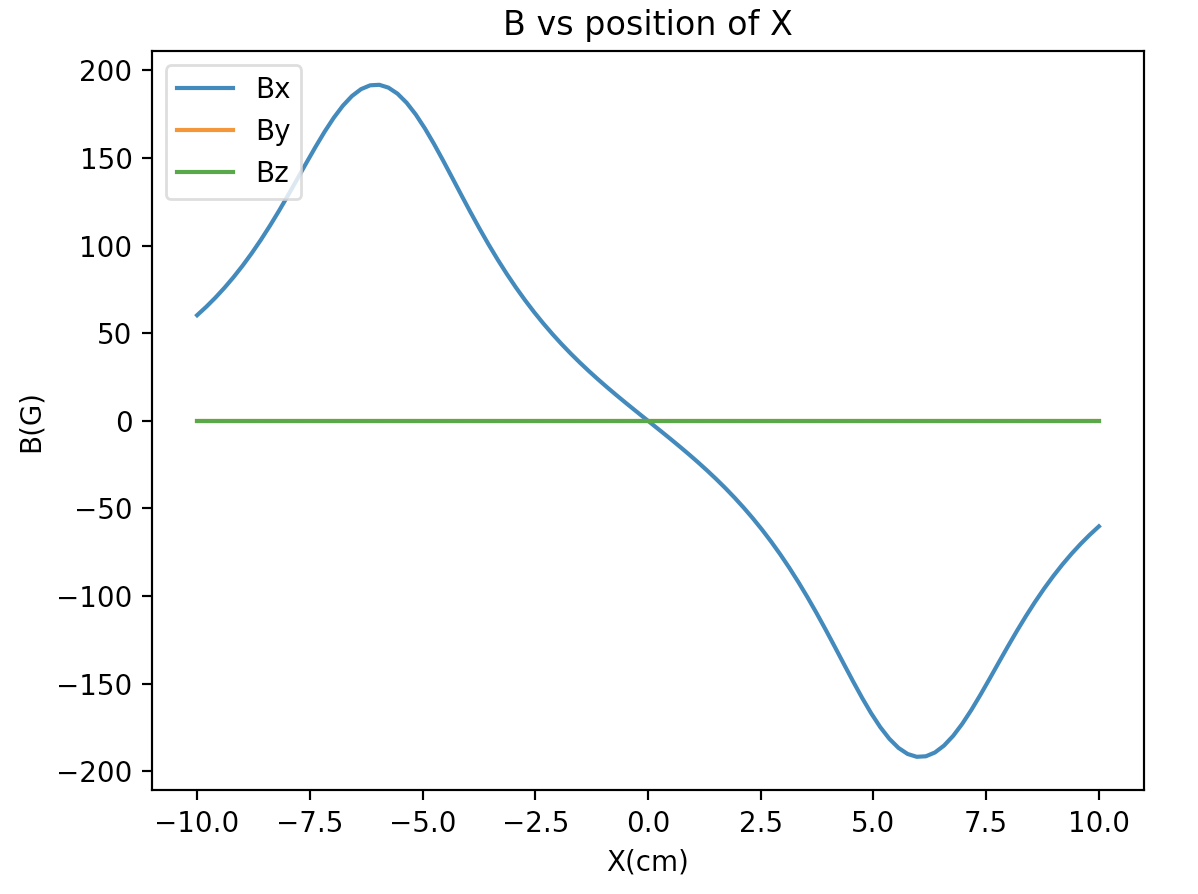
\includegraphics[scale=0.45]{OurBx}
	\caption{In our lab, components of B to x, y and z directions along x-axis}
\end{figure*}

\begin{figure*}[h]
	\centering
	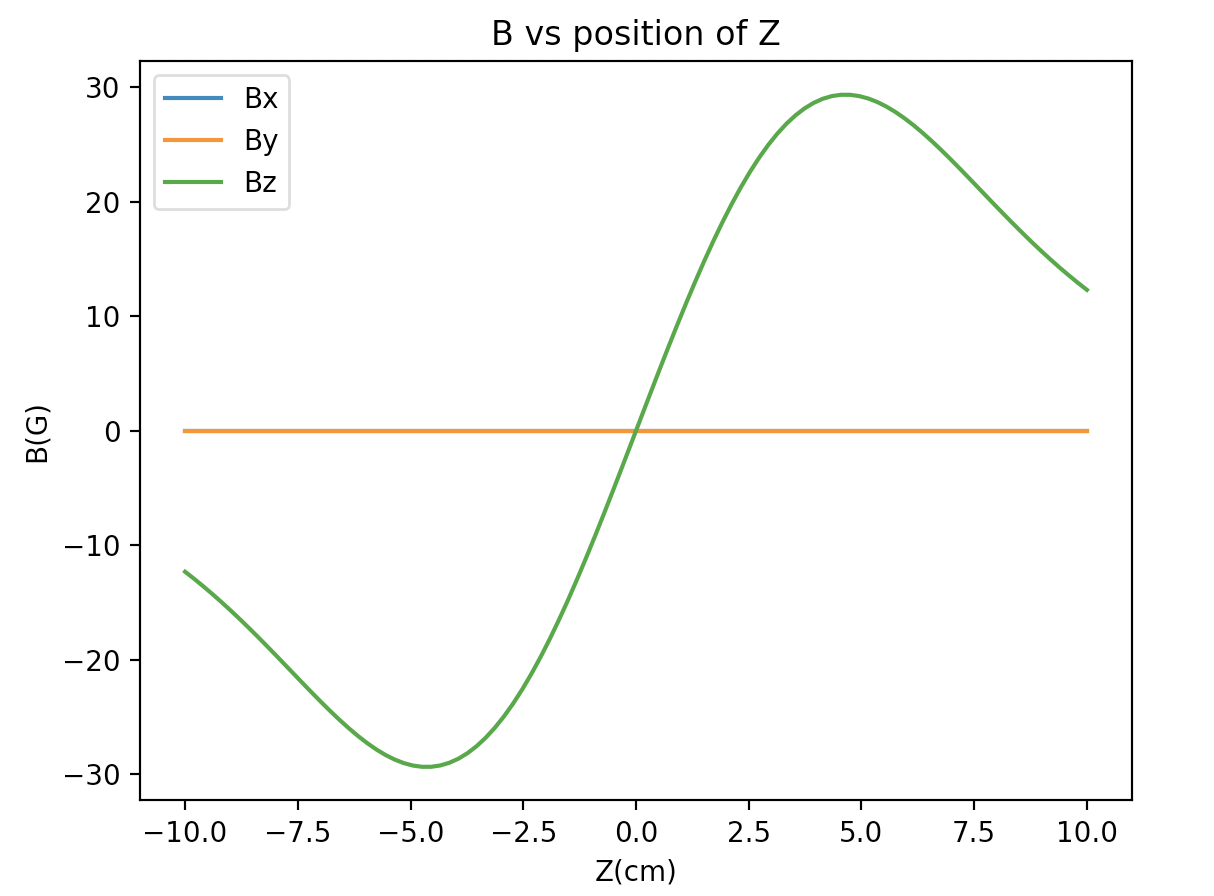
\includegraphics[scale=0.45]{OurBz}
	\caption{In our lab, components of B to x, y and z directions along z-axis}
\end{figure*}

\begin{figure*}[h]
	\centering
	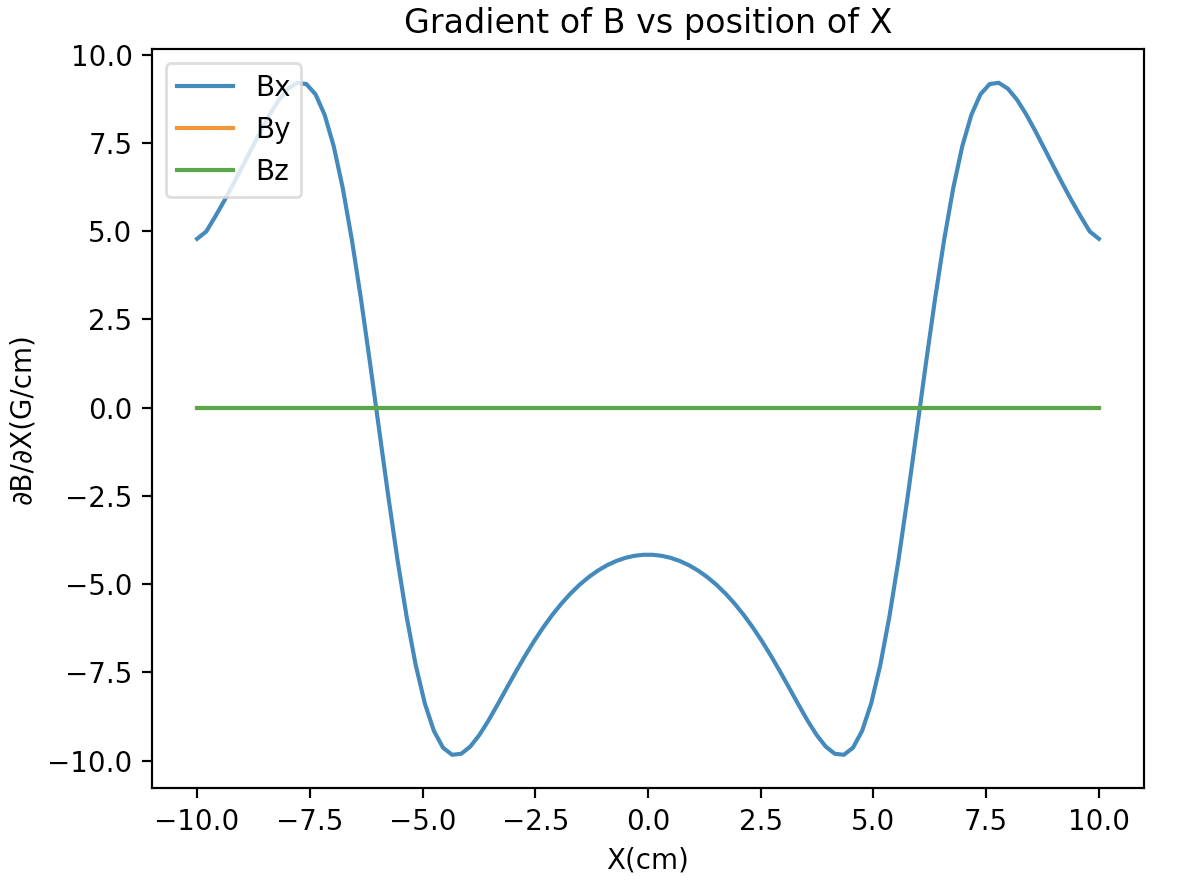
\includegraphics[scale=0.45]{OurGradX}
	\caption{In our lab, components of gradient of B to x, y and z directions along x-axis}
\end{figure*}

\begin{figure*}[h]
	\centering
	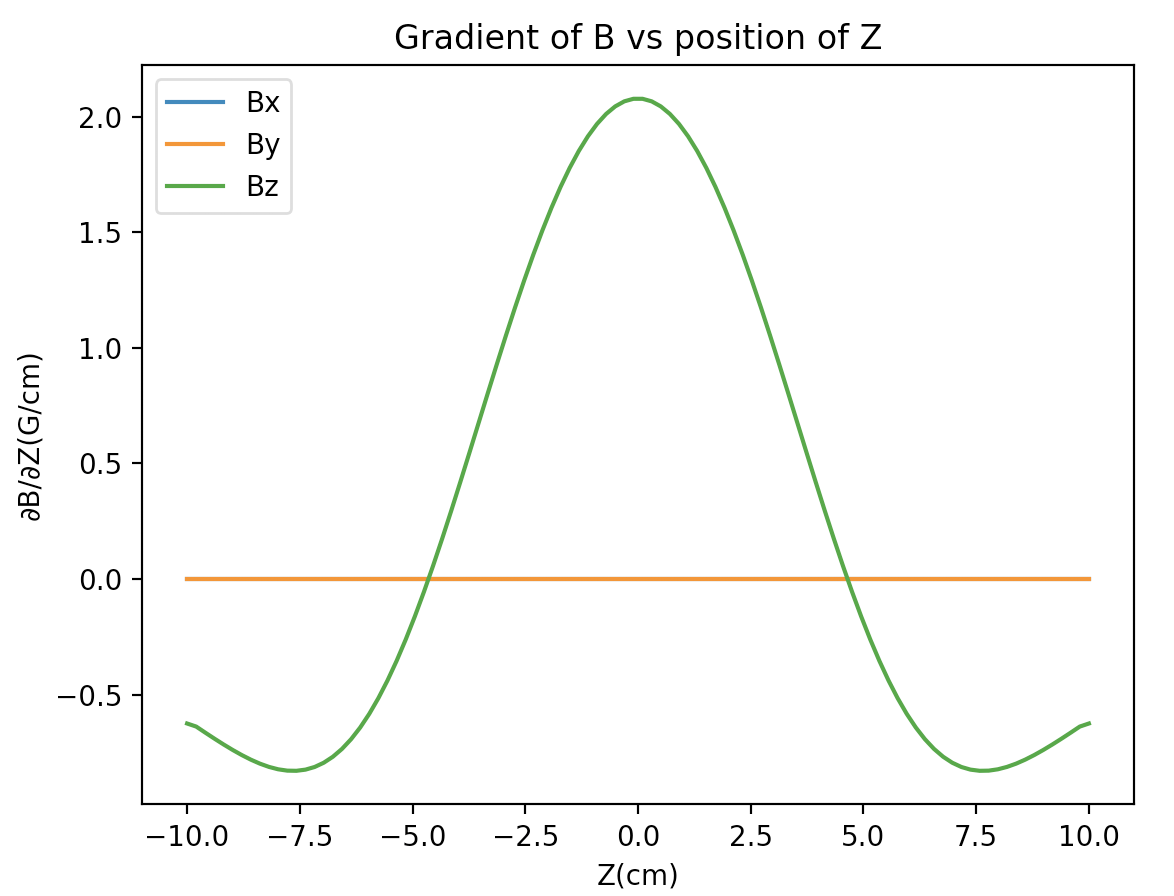
\includegraphics[scale=0.45]{OurGradZ}
	\caption{In our lab, components of gradient of B to x, y and z directions along z-axis}
\end{figure*}

\end{document}